\section{Projeto Geral}

O Projeto Geral consistirá em um drone quadrirrotor que deverá cumprir uma missão, assim como feito pela equipe em suas competições. O drone não será construído de fato, ele deve ser imaginado e simulado, para garantir o cumprimento de todas as etapas do projeto. A missão do Projeto Trainee EDRA 2025.1 é:

\begin{itemize}
    \item \textbf{Entrega Aérea de Suporte Humanitário com Reconhecimento de Base por QR Code}
    
    \textbf{Objetivo geral:} \\
    Executar uma missão autônoma com um drone que decola de uma base inicial, realiza navegação guiada por visão computacional, identifica um ponto de apoio através de QR code e realiza a entrega de um suporte humanitário, pousando com segurança ao final da missão.
    
    \begin{itemize}
        \item \textbf{Etapas detalhadas da missão:}
        
        \begin{enumerate}
            \item \textbf{Posicionamento inicial:}
            \begin{itemize}
                \item O drone estará inicialmente pousado sobre uma pequena plataforma ou caixa elevada, que deve ser segurada manualmente ou fixada no local de partida.
                \item O drone estará carregando um pacote representando suporte humanitário, que pode simbolizar água, medicamentos ou mantimentos.
            \end{itemize}
            
            \item \textbf{Decolagem:}
            \begin{itemize}
                \item O drone deve realizar uma decolagem vertical estável e segura, atingindo uma altura pré-definida (ex: 1,5 metros) para iniciar a missão.
            \end{itemize}
            
            \item \textbf{Navegação até o ponto de reconhecimento:}
            \begin{itemize}
                \item No chão haverá uma linha azul contínua {\color{red} com 20 cm de largura}, que poderá servir como rota visual de navegação.
                \item {\color{red}O drone deverá alcançar o ponto ao final do trajeto dessa linha azul para realizar a próxima etapa da missão, para isso poderá utilizar visão computacional para detectar e segui-la.}
            \end{itemize}
            
            \item \textbf{Leitura do QR Code de missão:}
            \begin{itemize}
                \item Ao final da linha azul, haverá um QR code visível contendo um número de 1 a 3, que indica qual base deve receber o suporte humanitário.
                \item O drone deve parar, ler o QR code, interpretar corretamente o número da base-alvo e armazenar essa informação para a próxima etapa.
            \end{itemize}
            
            \item \textbf{Identificação das bases:}
            \begin{itemize}
                \item À frente do ponto de leitura estarão posicionadas três bases {\color{red}cada uma na sua zona distinta (tal que alguma específica será apontada como certa pelo QR Code), cada uma com um padrão distinto visualmente identificável.}
                \item {\color{red}O drone deve identificar visualmente a base apontada como certa e se posicionar de forma precisa sobre ela, cujo código corresponde ao do QR code lido anteriormente.}
            \end{itemize}
            
            \item \textbf{Entrega do suporte humanitário:}
            \begin{itemize}
                \item Estando posicionado sobre a base correta, o drone deve realizar a liberação controlada do pacote de suporte humanitário diretamente sobre o alvo.
                \item A liberação deve ocorrer com o drone estabilizado e dentro da zona de entrega, simulando uma entrega precisa em um cenário de assistência real.
            \end{itemize}
            
            \item \textbf{Pouso:}
            \begin{itemize}
                \item Após a entrega, o drone deve se deslocar até uma área de pouso segura, que pode ser o ponto inicial ou um local previamente definido.
                \item O drone então realiza um pouso controlado e seguro, encerrando a missão.
            \end{itemize}
        \end{enumerate}
        
        \item \textbf{Objetivos avaliados na missão:} 
        \begin{itemize}
            \item Decolagem e pouso seguros e controlados
            \item Navegação visual por linha de referência
            \item Leitura correta do QR code {\color{red}e comportamento correspondente ao indicado pelo número lido}
            \item {\color{red}Identificação e} posicionamento preciso sobre a base correta
            \item Liberação eficaz da carga de suporte humanitário
            \item Autonomia na execução da missão com base em dados extraídos durante o voo
        \end{itemize}
    \end{itemize}

    \item {\color{red} Propriedades da caixa:
    
    \begin{itemize}
        \item Massa: 400 (g)
        \item Dimensões: 20x20x20 (cm)
    \end{itemize}}
\end{itemize}

Ademais, conforme dito na introdução, deverá ser produzido um relatório técnico final. Dessa forma é recomendável a leitura do livro Introduction to Multicopter Design and Control, de Quan Quan, além de outras fontes, citadas no final desse documento.

{\color{red}
\subsection{Especificações Detalhadas do Ambiente e Elementos de Missão}

O ambiente da missão é um espaço externo plano, quadrado, com dimensões de 30 metros por 30 metros e altura máxima operacional de 10 metros. O solo é de grama baixa, sem obstáculos, oferecendo textura visual, mas sem referências adicionais além dos elementos da missão descritos a seguir:

\begin{itemize}
    \item \textbf{Linha de Navegação:} Uma linha azul contínua, com largura de 20 cm, está desenhada no chão. Ela serve como referência visual para navegação do drone, podendo apresentar curvas suaves, mas sem ângulos retos ou loops. O comprimento da linha varia entre 5 e 15 metros.
    \item \textbf{QR Code:} Ao final da linha azul, há um QR Code de 100 cm de lado, posicionado no chão. O código contém um número de 1 a 3, indicando qual base de entrega deve ser selecionada pelo drone. O drone deve parar, ler e interpretar corretamente o QR Code para determinar a base-alvo.
    \item \textbf{Bases de Entrega:} Existem três bases de entrega, cada uma posicionada em uma zona (quadradas com 3 metros de lado) específica em relação ao QR Code:
    \begin{itemize}
        \item Zona 1: Centralizada 3 metros ao norte e 4 metros a oeste do QR Code
        \item Zona 2: Centralizada 5 metros ao norte do QR Code
        \item Zona 3: Centralizada 3 metros ao norte e 4 metros a leste do QR Code
    \end{itemize}
    Cada base possui uma figura geométrica regular e uma cor distinta (ver imagem abaixo), inscrita em uma circunferência de 80 cm de diâmetro, dentro de uma base quadrada de 80 cm de lado. As cores são especificadas em RGB (Hexadecimal) e as formas são regulares e facilmente distinguíveis por visão computacional.
\end{itemize}

\begin{figure}[H]
    \centering
    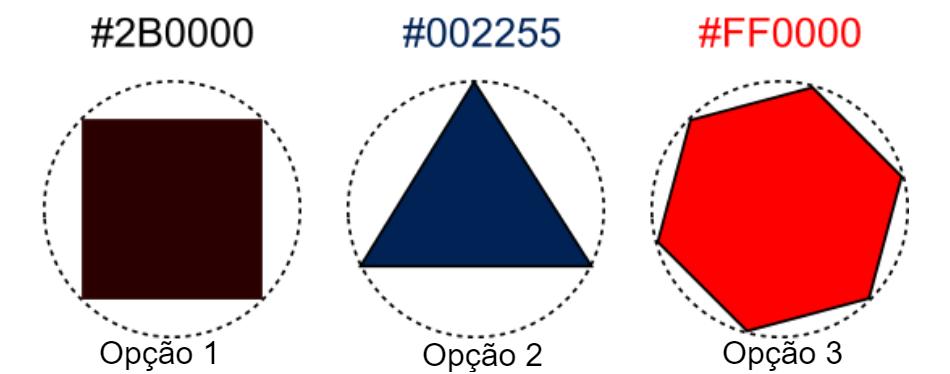
\includegraphics[width=0.8\textwidth]{Editáveis/opcoes_de_bases.png}
    \caption{\color{red}Opções de bases de entrega: cada base possui uma cor e forma geométrica distinta, conforme especificado.}
    \label{fig:opcoes_bases}
\end{figure}

\begin{figure}[H]
    \centering
    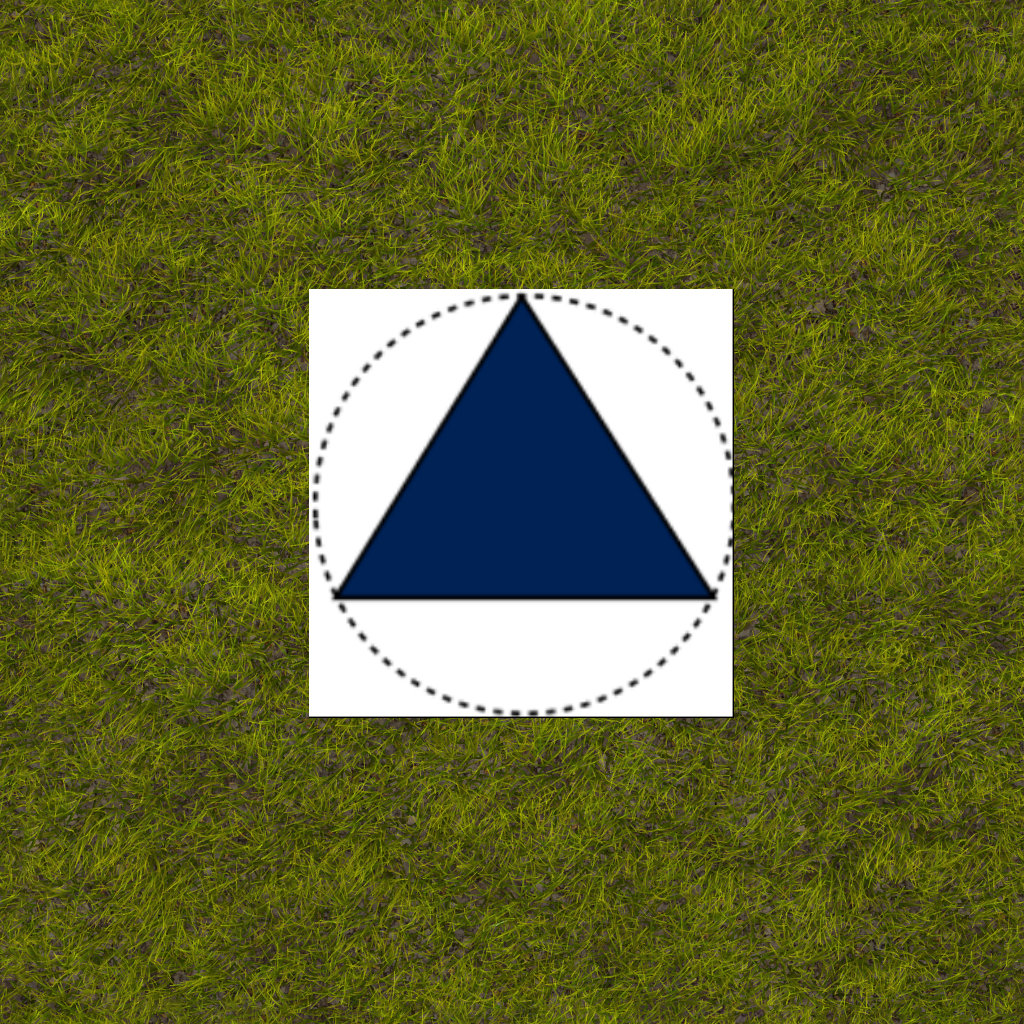
\includegraphics[width=0.4\textwidth]{Editáveis/base_na_grama.png}
    \caption{\color{red}Exemplo de base posicionada sobre o solo de grama. O círculo pontilhado é apenas referência para reprodução e não faz parte da base real.}
    \label{fig:base_exemplo}
\end{figure}

O ambiente não possui obstáculos móveis ou fixos além dos elementos descritos, o chão de grama oferece textura visual, mas sem referências adicionais.
}